\documentclass[../main.tex]{subfiles}
\begin{document}

\chapter[A gene-based association method for mapping traits]{A 
	gene-based association method for mapping traits using reference 
	transcriptome data}
\labch{gamazon2015}

\extauth{Eric R Gamazon, Heather E Wheeler, Kaanan P Shah, Sahar V 
Mozaffari, Keston Aquino-Michaels, Robert J Carroll, Anne E Eyler, 
Joshua C Denny, GTEx Consortium, Dan L Nicolae, Nancy J Cox \& Hae Kyung 
Im; Nature Genetics 2015}

\begin{external_abstract}{title=\textit{Abstract}}
Genome-wide association studies (GWAS) have identified thousands of 
variants robustly associated with complex traits. However, the 
biological mechanisms underlying these associations are, in general, not 
well understood. We propose a gene-based association method called 
PrediXcan that directly tests the molecular mechanisms through which 
genetic variation affects phenotype. The approach estimates the 
component of gene expression determined by an individual's genetic 
profile and correlates \enquote{imputed} gene expression with the 
phenotype under investigation to identify genes involved in the etiology 
of the phenotype. Genetically regulated gene expression is estimated 
using whole-genome tissue-dependent prediction models trained with 
reference transcriptome data sets. PrediXcan enjoys the benefits of 
gene-based approaches such as reduced multiple-testing burden and a 
principled approach to the design of follow-up experiments. Our results 
demonstrate that PrediXcan can detect known and new genes associated 
with disease traits and provide insights into the mechanism of these 
associations.
\end{external_abstract}

\section{Introduction}

% GWAS needs large sample size because the effects are small. sequencing 
% of large sample size is unfeasible.

Albeit it is accepted that in the majority of cases the biological role 
of variants associated to diseases is regulatory, as confirmed by the 
fact that many such variants are linked to eQTL and fall in regions that 
are epigenetically marked as regulatory, GWAS results remain mainly 
uncharacterised from a functional point of view, and are only able to 
explain a little proportion of phenotypic variance. The wealth of 
biological data that is now being released by large-scale consortia 
provides an unprecedented opportunity to integrate information and 
obtain insight into the genetic and biological processes underlying 
disease susceptibility\sidenote[][-3cm]{Some of these consortia, whose 
data sets have been used by Gamazon \etal, are the following.
\begin{description}
	\item[ENCODE.] The focus is on the systematic functional annotation 
of each element of the human genome.
	\item[GEUVADIS.] This project endeavours to uncover functional 
variation in humans through the study of how genetic variants affect 
gene expression.
	\item[DGN.] Variants regulating gene expression, splicing and 
allelic expression are detected.
	\item[Braineac.] The authors find eQTL in ten human brain regions.
	\item[GTEx Project.] Its aim is to collect data on genotype and gene 
expression levels of a number of tissues from postmortem samples.
\end{description}
}.

This seminal article is based on two key ideas: first, genetic variants 
most often impact gene expression, as shown by the many eQTL studies; 
second, SNP aggregation methods that combine many variants in a 
biologically meaningful way have the potential to improve GWAS results. 
In particular, the authors propose to group together all the SNPs that 
regulate the expression of a given gene. One advantage of this approach, 
which they called PrediXcan, is that statistical tests performed on 
group of SNPs are more powerful than those performed on each and every 
SNP, due to less multiple testing; besides, by choosing the gene as a 
grouping unit, information about the directionality of the effect is 
intrinsically provided, \ie it is possible to say whether the disease is 
associated to an increase or a decrease in the gene's expression. 
Additionally, from a functional point of view a gene is much more 
interpretable than a simple genetic polymorphism.

\section{Imputation of gene expression}

The main goal is to provide a framework to better interpret GWAS 
results. However, in a typical GWA study the individuals are simply 
genotyped with a SNP microarray, and expression data are completely 
missing. Therefore, gene expression has to be predicted by exploiting 
the knowledge of expression quantitative trait loci. Here, a linear 
regression model is fitted on a reference transcriptome data set, where 
both genotype and expression data are available; then it is applied on 
the individuals of a GWAS, for which only genotype data is collected, in 
order to predict expression levels.

The first assumption here is that gene expression can be decomposed into 
three components: a genetically regulated expression (GReX), a 
phenotype-influenced expression, and an environment-determined component 
(\reffig{gamazon2015/1}). Some phenotype, including many diseases, can 
indeed influence gene expression, but, as we shall see in a moment, 
since the models that predict gene expression are trained on healthy 
individuals from reference transcriptome experiments, they already 
exclude that component from what they predict.

\begin{figure}
	\centering
	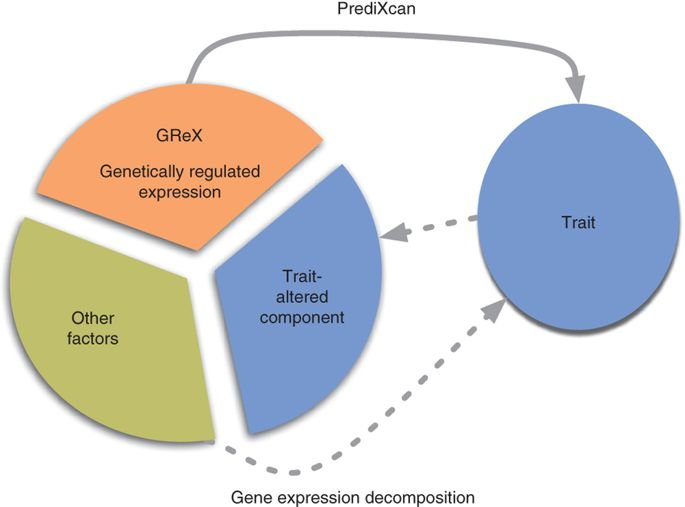
\includegraphics[width=0.8\textwidth]{gamazon2015/1-expression_decomposition}
	\caption{Gene expression can be decomposed into three components}
	\labfig{gamazon2015/1}
\end{figure}

The prediction relies on data sets where both genotype and expression 
are present, such as the aforementioned GEUVADIS and GTEx projects, and 
the model is additive (\reffig{additive_model}), meaning that a given 
variant in a homozygous individual is supposed to have twice the effect 
of that same variant in an heterozygous individual. This is surely an 
oversimplification, for it does not take into account three biologically 
important effects ---epistasis, dominance and penetrance---, but an 
additive model is much simpler to implement. Moreover, the model 
performs multiple linear regression, which is a first attempt to 
quantitatively model the interactions among \textit{many} genetic 
variants: indeed, it may well be that a given phenotype is influenced by 
a \textit{combination} of SNPs rather than a single SNP. The purpose of 
this regression model is to find for each SNP the coefficient of which 
gene expression is altered by a copy of that SNP. Once the coefficients 
have been estimated, the genetically regulated component of gene 
expression can be predicted starting only from the genotype of an 
individual; the predicted GReX is denoted as $\widehat{GReX}$.

\begin{marginfigure}[-7cm]
	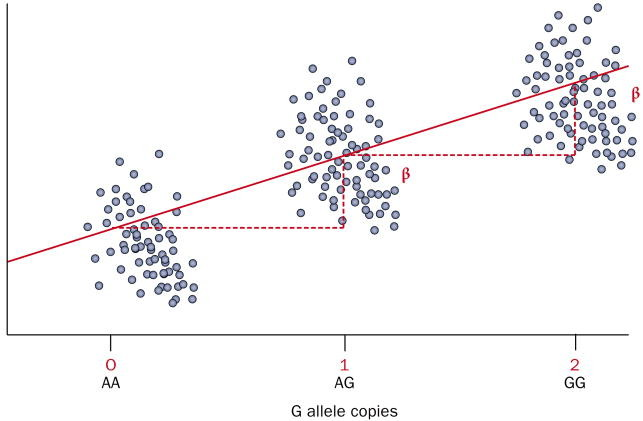
\includegraphics{gamazon2015/ext-additive_genetic_model}
	\caption{An example of additive model for one SNP; Gamazon \etal 
extended it for several SNPs. Image adapted from Conall M. O'Seaghdha 
and Caroline S. Fox, \enquote{Genome-wide association studies of chronic 
kidney disease: what have we learned?}}
	\labfig{additive_model}
\end{marginfigure}

They thus generated predictDB, which stores the coefficients of which 
each SNP influence the GReX. By using healthy individuals from reference 
transcriptome and genome data sets, they disregard the 
disease-determined component of gene expression, and by using a 
regression model, they disregard the random environmental component. It 
is now possible to \enquote{impute} the transcriptome of an individual 
from its genotype, just like it is possible to impute unknown genetic 
variants in an individual from its known genotyped variants.

\begin{figure}
	\centering
	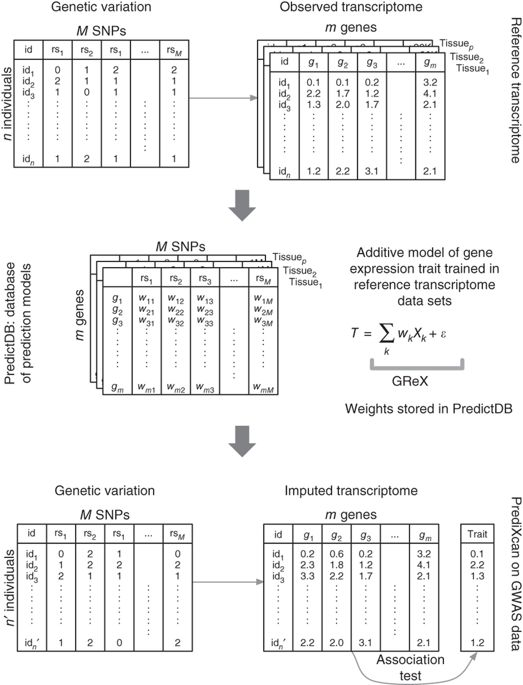
\includegraphics[width=0.85\textwidth]{gamazon2015/2-grex_estimation}
	\caption{The framework to estimate the coefficient by which each SNP 
alters the expression of a gene.}
	\labfig{gamazon2015/2}
\end{figure}

The regression model employed can be summarised with the following 
equation (referring to \reffig{gamazon2015/2}):

\begin{equation}
	T = \sum_{k=1}^{M}w_k X_k + \epsilon
\end{equation}

where T is the expression of a given gene in a given tissue, $w_k$ is 
the weigth (or the effect size) of SNP $k$ in influencing the expression 
of that gene, $X_k$ is the number of reference alleles of SNP $k$ in all 
the data set, and $\epsilon$ is a residual error. Only SNPs falling 1Mb 
within the gene's start or end were considered. To fit this model, the 
authors tried various types of regression methods ---lasso, elastic net 
and polygenic scrores---, but in the end settled to elastic 
net\sidenote{In general, elastic net is used for two reasons: first, 
when the number of predictors is large, especially if compared to the 
number of samples; and second, to avoid overfitting.} (with the 
parameter $\alpha = 0.5$), whose main advantage is the 
\enquote{automatic} selection of the most important regressors. In this 
case, the SNPs that have a small influence on gene expression, or that 
are correlated to another SNP that can explain more variation in gene 
expression, are neglected. 10-fold cross-validation\sidenote{In $k$-fold 
cross-validation, the dataset is split in $k$ portions, and for each 
part, the model is trained on the remaining $k-1$ parts, then the $R^2$ 
of the predicted and real values is calculated on the selected part. The 
average of the $R^2$ is finally reported.} was used to asses the 
predictive performance.

Having seen the general method, we now turn to the actual protocol 
followed by the authors.

From DGN, they obtained whole-blood RNA-seq and genome-wide genotype 
data for 922 European individuals, normalised and filtered to retain 
only SNPs with MAF > 0.05, in Hardy-Weinberg equilibrium and univoquely 
mapped onto a strand. The SNPs that were not genotyped were 
imputed\sidenote{Genome imputation is a routinely-used method to 
estimate the genotype of an individual at loci that were not analysed, 
basing on known linkage disequilibrium information in a reference 
population}. This data set was used to train the predictive models.

From GEUVADIS, normalised RNA-seq data from lymphoblastoid cell lines 
established from 421 individuals was downloaded; genotype data was also 
available for the same individuals, since they were part of the 1000 
genomes project as well. This data set was used for the validation of 
the models (\reffig{gamazon2015/4}).

\begin{figure}
	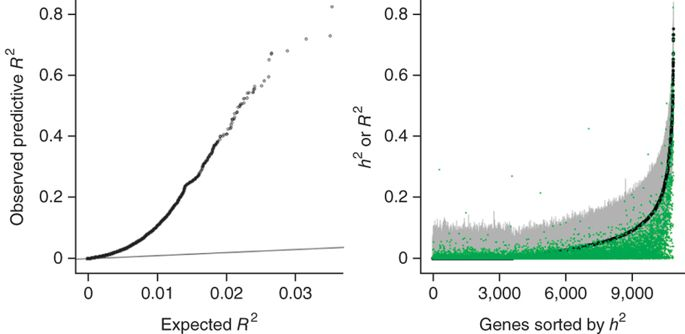
\includegraphics{gamazon2015/4-prediction_performance}
	\caption{The performance in the GEUVADIS data set of the elastic net 
model trained on the DGN data set, showed by a quantile-quantile plot 
(left) and a distribution of $R^2$ (right).}
	\labfig{gamazon2015/4}
\end{figure}

In the quantile-quantile plot of \reffig{gamazon2015/4} each point 
represents an expression value; on the $x$-axis it is reported the $R^2$ 
that would be expected if the null hypothesis were true (\ie, if there 
were no correlation between predicted and observed expression values), 
while on the $y$-axis there is the observed $R^2$. A 45\textdegree\ line 
is displayed in gray: the farther the points are from that line, the 
more different the two distributions of $R^2$ are. Since in this plot 
the distributions are fairly discordant, we can reject the null 
hypothesis and state that the correlation between predicted and real 
expression is quite good. In the scatter plot to the right, the 
distribution of $R^2$ is plotted; the black line represents 
heritability, a threshold which theoretically the $R^2$ cannot pass, as 
explained in the next section.

RNA-seq data from GTeX, normalised and adjusted for the most common 
covariates such as sex, was used to test the predictive performance of 
the model in different tissues. Surprisingly, the model was able to 
predict gene expression quite accurately in tissues other than the 
blood, even though it was trained on blood expression data.

\section{Heritability of gene expression}
\labsec{heritability}

Heritability is an important idea in genetics and is especially relevant 
in the scope of association studies, therefore we dedicate some space to 
its analysis.

Many traits vary among the individuals of a population: height and hair 
colour are obvious ones, but for instance also disease status (or the 
liability to it) can be considered a phenotypic trait. The heritability 
of a trait is the proportion of trait variance which can be explained by 
the genetic variance among the individuals of the population. In order 
not to underestimate heritability, only genetic variance at loci 
associated to the phenotype must be taken into account. Heritability 
does not deal with the influence of genes in the development of the 
trait, but rather is concerned with the role of genetic 
\textit{variation} in determining phenotypic variation. There are two 
definitions of heritability:

\begin{description}
	\item[Narrow sense heritability,] or $h^2$, is the heritability due 
to additive genetic factors (see \reffig{additive_model} and related 
discussion).
	\item[Broad sense heritability,] or $H^2$, is the heritability due 
to all genetic factors, taking into account dominance and gene-gene 
interactions.
\end{description}

\marginnote[-1.5cm]{If we assume that $P = G + E$, where $P$ is the 
	phenotype, $G$ the genetics, $E$ the environment, then phenotypic 
	variance can be expressed as follows:
\begin{equation*}
	Var(P) = Var(G) + Var(E) + 2 Cov(G,E)
\end{equation*}
and, assuming the independence of genetics and environment,
\begin{flalign*}
	&H^2 = Var(G) / Var(P)
	&\\
	&h^2 = Var(A) / Var(P)
\end{flalign*}
}

Usually, the first definition is used, and it is a reasonable 
approximation, for in the majority of case, alternate alleles are 
homozygous only in a minority of individuals due to their low frequency, 
hence the effects of dominance or epistasis manifest only 
rarely\autocite{Visscher2008}.

There are many ways to estimate narrow-sense heritability. One is in 
selective breeding, where the heritability is the proportionality 
coefficient between the intensity of the applied selective pressure, 
$S$, and the response to selection, $R$ (\reffig{breeders}). In other 
words, $R = h^2 S$, wihch is the famous breeder's equation. The larger 
the heritability, the greater the response to selection.

\begin{figure}
	\centering
	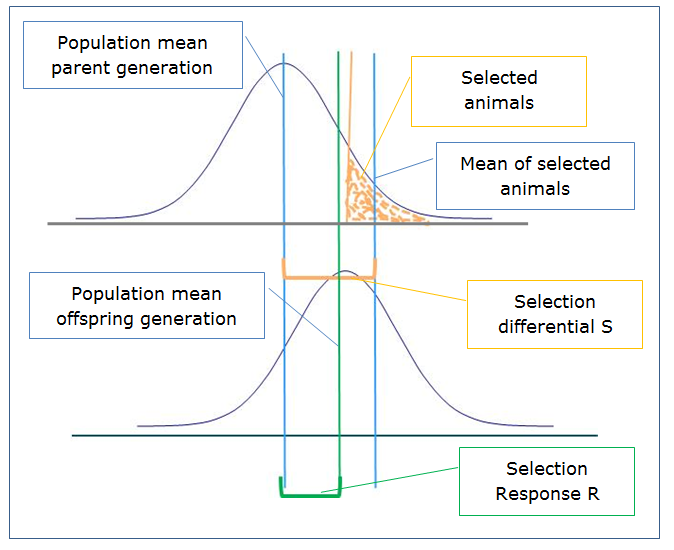
\includegraphics[width=0.75\textwidth]{gamazon2015/ext-breeders}
	\caption{The breeder's work. Source: 
\url{https://wiki.groenkennisnet.nl/}}
	\labfig{breeders}
\end{figure}

Another way to interpret heritability in the narrow sense is the 
plotting of the averaged trait in the two parents versus the trait in 
their offspring. In principle, if genes determine variations in 
phenotypes, then offspring should be more similar to their parents than 
to unrelated individuals. This can be expressed as a correlation between 
parents and offspring (\reffig{parents_offspring}). In general, $h^2$ is 
the slope of the regression line of the phenotypes of offspring and 
parents. This, however, is valid only if the environment is not shared 
between relatives more than it is shared between unrelated people.

\begin{figure}
	\centering
	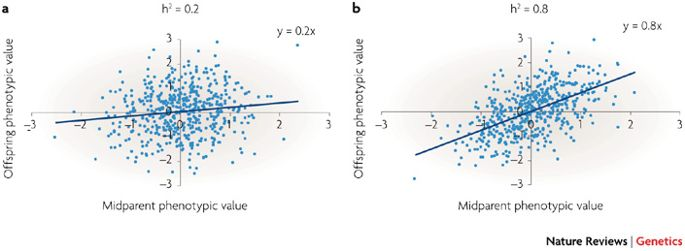
\includegraphics{gamazon2015/ext-parents_offspring}
	\caption{Parents-offspring regression. Source: 
\textcite{Visscher2008}}
	\labfig{parents_offspring}
\end{figure}

Returning to the paper by Gamazon \etal, they rightly claim that 
heritability is an upper bound to how well the trait can be associated 
to the genotype. A high heritability means that the parents' trait can 
predict the offspring trait, or, equivalently, since this predictability 
is due to genetic factors, that people with a similar genotype will have 
a similar phenotype (indeed, $h^2$ is precisely the correlation between 
the phenotypes in parents and offspring).

The heritability of gene expression in DGN cells was computed, resulting 
in an average value of 0.153, whereas the average 10-fold 
cross-validation $R^2$ between the $\widehat{GReX}$ and the real 
expression was 0.137. \reffig{gamazon2015/3} reports the results of the 
cross-validation. Expression, contrary to other phenotypes, can be 
predicted very accurately from genotypes.

\begin{figure}
	\centering
	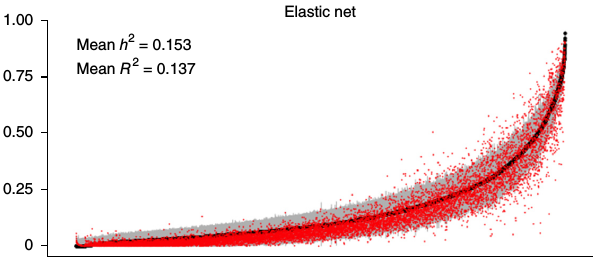
\includegraphics{gamazon2015/3-prediction_r2}
	\caption{$R^2$ (red) of $\widehat{GReX}$ versus observed expression; 
heritability (black) of gene expression. The fact that this two measures 
are so close indicates that the prediction of the expression works.}
	\labfig{gamazon2015/3}
\end{figure}

\section{Correlation between expression and phenotype}

In the second phase, the predicted $\widehat{GReX}$ is associated with 
the phenotypic status. To this aim, linear regression, logistic 
regression, Cox regression, or Spearman correlation (the latter is 
non-parametric) can be employed. For the results discussed in this 
article, logistic regression was chosen. Much like in a GWAS some 
variants are more frequent in cases than in controls, in a TWAS some 
genes will be more or less expressed in patients than healthy people.

This is the core part of a TWAS. It goes beyond genetic variants, and 
allows to explore the genetic basis of disease through the proxy of 
expression.

\section{Application of PrediXcan to WTCCC GWAS}

At last, the method was applied to seven autoimmune diseases which had 
previously been the object of as many GWAS by the Wellcome Trust Case 
Control Consortium. They used DGN whole-blod elastic net prediction 
models to predict the expression in each WTCCC cohort, then correlated 
the predicted GReX with the disease status. After applying Bonferroni 
correction, 41 significant associations (P-value < 0.05) with 5 diseases 
were reported. Most of the significant associations were for autoimmune 
disease and were located in the extended MHC 
region\sidenote[][-2cm]{This region, located on chromosome 6, harbours 
	421 loci, including 252 expressed genes, 139 pseudogenes and 30 
		transcripts. Many of these loci are associated to diseases.}. 
Moreover, some genes were associated to multiple 
diseases\sidenote[][-0.5cm]{In these cases, what determines which 
disease shows up if the expression of that gene is altered in an 
individual? Perhaps the environment, or gene expression level. This is 
an example of the complexity of the situation: the relationship between 
genotype and phenotype is not biunivocal at all.} The majority of these 
associations were supported by previous evidence, and often they were 
enriched in known GWAS; but two completely novel disease-associated 
genes were also found: low expression of \textit{KCNN4} was associated 
with hypertension, and high expression of \textit{PTPRE} with bipolar 
disorder.

One of the most interesting features of this new approach is that not 
only can it provide association results, but also a directionality. As 
an example, \textit{PTPN22} expression was positively associated with 
rheumatoid arthritis and type 1 diabetes, and negatively associated with 
Crohn's disease.

The results of the associations with type 1 diabetes are reported in 
\reffig{gamazon2015/7}.

\begin{figure}
	\centering
	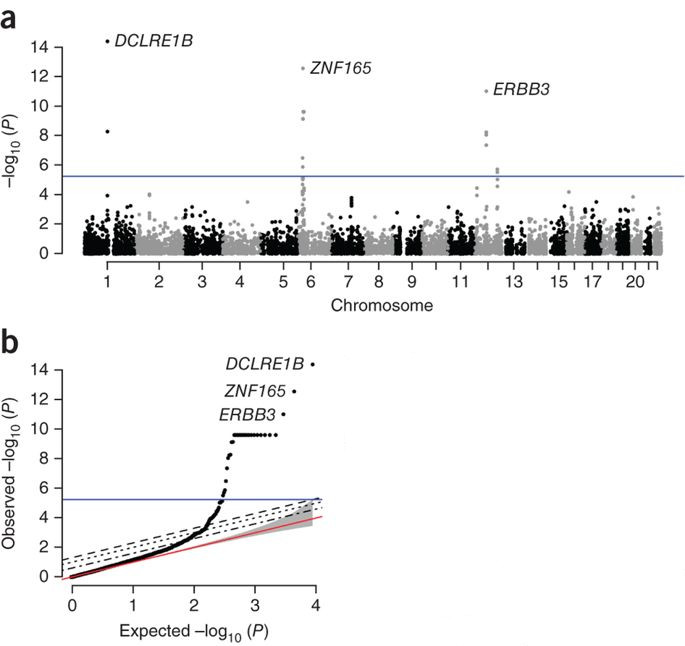
\includegraphics{gamazon2015/7-t1d_associations}
	\caption{(a) Manhattan plot of disease-gene associations P-values. 
(b) Q-Q plot of the same P-values. The top three genes are emphasised.}
	\labfig{gamazon2015/7}
\end{figure}

\section{Discussion}

General considerations on transcriptome-wide association studies are 
postponed until all the articles are discussed; in the discussion 
section of each paper, ideas about the particular article will be 
considered.

In this work, which can be regarded as the founder of the field of TWAS, 
the authors developed a framework to group together genetic variants, 
predict how such variants influence gene expression, and finally 
correlate gene expression to a disease. The last step was the real 
association study, whereas the imputation of gene expression was needed 
only because expression data are missing in GWAS samples.

This imputation step makes PrediXcan economic, in the sense that one 
only needs reference transcriptome and GWAS data, which are already 
available, to perform a TWAS; therefore, many existing GWAS dataset can 
be reanalysed \enquote{for free}. Nevertheless, due to privacy or 
logitic reasons, individual-level data\sidenote{That is, the genotype of 
each individual in the cohort.} for published genome-wide association 
studies are often unavailable. The article analysed in the next chapter, 
by Gusev \etal, shall eliminate this limitation.

The authors chose to use elastic net to predict gene expression, but 
argue that this expression might be biased, and that more sophisticated 
methods, like a combination of K nearest neighbours (KNN), elastic net 
and the use of genomic annotation, may perform better. Besides, we add 
that elastic net does not take into account biologically important 
concepts such as epistasis, dominance and penetrance.

The use of logistic regression to perform the association between 
expression and disease is arguable, too. For instance, another 
possibility could have been that not to model the disease status, which 
is a binary variable, but rather the liability to the disease, following 
what Vissher\autocite{Visscher2008} reported showing that this approach 
is able to explain a larger proportion of genetic variance.

When applied to real world GWAS, PrediXcan performed well. Most genes 
had already been found, but two novel ones were reported as well. The 
features of these two genes were not investigated, but in the next 
articles we shall see that outliers like these were found to be 
regulated by multiple causal SNPs, rather than one (\eg, see 
\refsec{allelic_heterogeneity}).

\end{document}
